\documentclass{article}
\usepackage{include/nips15submit_e,times}
\usepackage{hyperref}
\usepackage{url}
\usepackage[noend]{algpseudocode}
\renewcommand\algorithmicthen{}
\renewcommand\algorithmicdo{}
\usepackage{algorithm}
\usepackage{natbib}
\usepackage{graphicx}
\usepackage{array,booktabs}
\usepackage{amsmath, amssymb}


\definecolor{mydarkblue}{rgb}{0,0.08,0.45}
\definecolor{myfavblue}{rgb}{0.1176, 0.392, 1.0}
\hypersetup{
    colorlinks=true,
    linkcolor=mydarkblue,
    citecolor=mydarkblue,
    filecolor=mydarkblue,
    urlcolor=mydarkblue}

%\newcommand{\citep}{\cite}
%\newcommand{\citet}{\cite}

\newcommand{\vw}{\mathbf{w}}
\newcommand{\vx}{\mathbf{x}}
\newcommand{\vy}{\mathbf{y}}
\newcommand{\vv}{\mathbf{v}}
\newcommand{\vf}{\mathbf{f}}
\newcommand{\vg}{\mathbf{g}}
\newcommand{\vi}{\mathbf{i}}
\newcommand{\vr}{\mathbf{r}}
\newcommand{\vI}{\mathbf{I}}
\newcommand{\vzero}{\mathbf{0}}
\newcommand{\ones}[1]{\mat{1}_{#1}}
\newcommand{\eye}[1]{\mat{E}_{#1}}
\newcommand{\tra}{^{\mathsf{T}}}
\newcommand{\vect}[1]{{\bf{#1}}}
\newcommand{\mat}[1]{\mathbf{#1}}
\newcommand{\pderiv}[2]{\frac{\partial #1}{\partial #2}}
\newcommand{\npderiv}[2]{\nicefrac{\partial #1}{\partial #2}}
\newcommand{\argmin}{\operatornamewithlimits{argmin}}
\newcommand{\argmax}{\operatornamewithlimits{argmax}}
\newcommand{\expect}{\mathbb{E}}
\newcommand{\expectargs}[2]{\mathbb{E}_{#1} \left[ {#2} \right]}
\newcommand{\var}{\mathbb{V}}
\newcommand{\varL}{\mathcal{L}}
\def\iid{i.i.d.\ }
\def\simiid{\overset{\mbox{\tiny iid}}{\sim}}
\newcommand{\defeq}{\mathrel{:\mkern-0.25mu=}}
\newcommand{\Normal}{\mathcal{N}}
\newcommand{\Nt}[3]{\mathcal{N}\!\left(#1 \middle| #2,#3\right)}
\newcommand{\N}[2]{\mathcal{N}\!\left(#1,#2\right)}
\DeclareMathOperator{\KLop}{KL}
\newcommand{\KL}[2]{\KLop \left(#1 \middle \| #2 \right)}



% Symbol definitions.
\newcommand{\distinit}{q_0(\params, \vv)}
\newcommand{\data}{\vx}

%% \newcommand{\params}{\vx}
\newcommand{\params}{\mathbf{\theta}}
\newcommand{\trans}{T}
\newcommand{\paramsrv}{\vX}  % Random variable.
\newcommand{\numsteps}{T}
\newcommand{\decay}{\gamma}
\newcommand{\decays}{{\boldsymbol{\decay}}}
\newcommand{\stepsize}{\alpha}
\newcommand{\stepsizes}{{\boldsymbol{\stepsize}}}
\newcommand{\gradparams}{\nabla L(\params_t, t)}
\DeclareMathOperator{\SGD}{SGD}
\newcommand{\entropy}{S}
\newcommand{\pun}{{\tilde p}}
\newcommand{\jointdist}{p(\params , \data)}
\newcommand{\posterior}{p(\params | \data)}
\newcommand{\subjointdist}[2]{p_{#1}(\params_{#2} , \data)}
\newcommand{\subjointdistminibatch}[1]{\tilde{p}(\params_{#1} , \data)}
\newcommand{\reals}{\mathbb{R}}
\newcommand{\bigo}[1]{\mathcal{O}\left(#1\right)}
\newcommand{\trace}[1]{\text{Tr}\left[#1\right]}
\newcommand{\loss}{L(\params)}


\makeatletter
\renewcommand*{\@fnsymbol}[1]{\ensuremath{\ifcase#1\or \dagger\or \ddagger\or
   \mathsection\or \mathparagraph\or \|\or **\or \dagger\dagger
   \or \ddagger\ddagger \else\@ctrerr\fi}}
\makeatother

\title{Langevin Flow for Gradient-based Nonparametric Variational Inference}

\author{}

%\nipsfinalcopy
\begin{document}
\maketitle

\begin{abstract}
Variational autoencoders are a family of inference strategies that use a recognition network to quickly approximate conditional posteriors.
Recently, these methods have been extended to produce non-parametric approximating distributions that can approach the true conditional posterior arbitrarily closely.
However, existing techniques require parameterization and optimization of either the recognition network, or the entropy estimator required for the variational lower bound.
We develop a family of nonparametric variational posteriors defined as the output of stochastic gradient descent with noise, also known as Langevin dynamics.
These dynamics admit a parameter-free entropy lower bound, and adapt to the true posterior asymptotically without tuning.
These properties make the Langevin flow sampler suitable for inference in high-dimensional spaces.
\end{abstract}

\section{Introduction}

[cite Shakir and Danilo] introduced the idea of using Langevin flows as an approximating family, but did not propose a lower bound.
[Maclaurin et al] developed a scalable unbiased lower bound estimate for the entropy implicitly defined by stochastic gradient descent dynamics.
We combine this bound with the entropy power inequality [cite] to extend it to the case where noise is added at each step.

\begin{figure}
\centerline{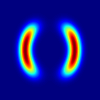
\includegraphics[height=0.34\textwidth, height=0.4\textwidth]{../montage/two_moons_density.png}
\hspace{2em}
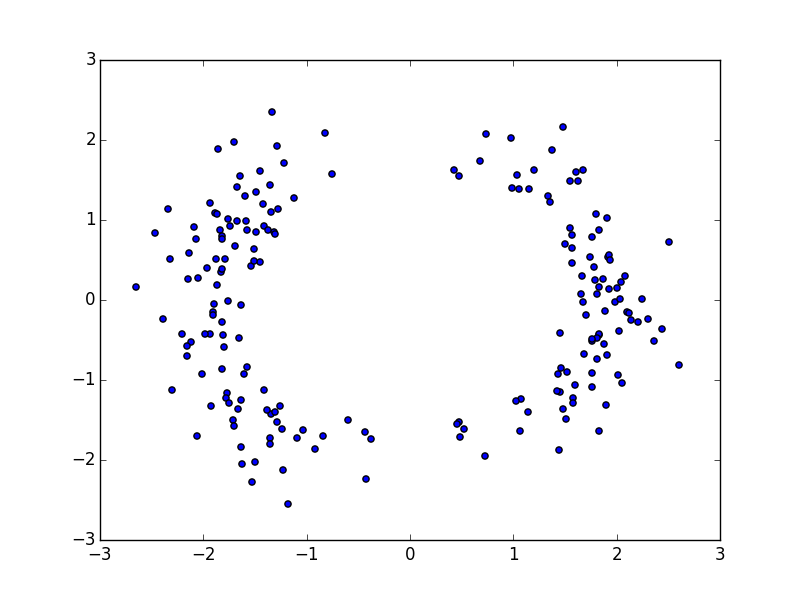
\includegraphics[height=0.4\textwidth, height=0.4\textwidth]{../experiments/4-test-flows/2-langevin/approximating_dist.png}}
\caption{\emph{Left}: Two moons toy density.
\emph{Right}: Samples from Langevin flows approximating density.}
\label{fig:toy examples}
\end{figure}

\section{Langevin Flow}

[Note: we can also use Langevin flow with SGD, while Betancourt's paper implies that we can't use HMC very effectively with stochastic gradients.  So we could use it for doubly-intractable distributions where we only get stochastic estimates of the likelihood.]

\begin{algorithm}[t]
   \caption{Langevin flow with entropy estimate}
   \label{alg:langevin-with-estimate}
\begin{algorithmic}[1]
	\State {\bfseries input:}
	Weight initialization scale $\sigma_0$, step size $\stepsize$,
	twice-differentiable negative log-likelihood $L(\params, t)$
	\State {\bfseries initialize} $\params_0 \sim \N{0}{\sigma_0 \vI_D}$
	\State {\bfseries initialize} $\entropy_{0} = \frac{D}{2} (1 + \log 2 \pi) + D \log\sigma_0$
	\For{$t=1$ {\bfseries to} $T$}
%		\State $\vg = \gradparams$             \Comment{Evaluate gradient}
%		\State $\vr \sim \N{0}{\vI_D}$         \Comment{Draw random direction}
%		\State $\vr\tra \left[ -2 \vr + 3 \left(  R1 - R2 \right) \right]$      \Comment{Estimate determinant}
		\State $\entropy_{t} = \entropy_{t-1} + \log \left| \vI - \stepsize H_{t-1} \right|$\Comment{Update entropy} \label{step:entropy-update}
		\State $\params_{t} = \params_{t-1} - \stepsize \gradparams$  \Comment{Update parameters}	
   \EndFor
   \State \textbf{output} sample $\params_T$, entropy estimate $\entropy_T$
\end{algorithmic}
\end{algorithm}


\section{Experiments}
\label{sec:experiments}


\paragraph{Binarized MNIST}

Results are summarized in Table~\ref{table:mnist results}.
%
\begin{table}
\begin{center}
\begin{tabular}{l|l}
Method & Nats \\
\midrule
Ours & Good \\
Theirs & Bad
\end{tabular}
\label{table:mnist results}
\caption{Nats per image.}
\end{center}
\end{table}

\paragraph{Software}
To compute our bounds, we required third-order gradient information.
For this, we used an automatic differentiation package for Python called Autograd (\url{github.com/HIPS/autograd)}.
This package handles standard Numpy~\citep{oliphant2007python} code, and can differentiate code containing while loops, branches, and indexing.

Code for all experiments is available at \url{github.com/HIPS/autopaint}.

\section{Limitations}
%In this section we detail some limitations of the neural fingerprint architecture used in this paper.

\paragraph{Computational cost}
Both HMC and Langevin flows require gradient evaluation of $p(x,z)$ at every step.


\paragraph{Limited adaptation to off-diagonal constraints}



\section{Related work}

\paragraph{Unrolled inference algorithms}
\citet{hershey2014deep} and others have noted that iterative inference procedures sometimes resemble the feedforward computation of a recurrent neural network.
One natural extension of these ideas is to parameterize each inference step, and train a neural network to approximately match the output of exact inference using only a small number of iterations.


\section{Conclusion}

\subsection*{Acknowledgments}
We thank Dougal Maclaurin for helpful discussions.

\bibliography{references}
\bibliographystyle{include/icml2015}
\end{document}